\documentclass[10pt]{article}
\usepackage{icmlko}

\icmlmeta{IP 파운데이션 월드모델}{42}{눈금이 맞았을 뿐 신호는 그대로였다}{노트 41을 한 노트 만에 철회한다 --- 순열 검정이 MAE 기준이라 축소를 개선으로 읽었다}

\begin{document}

\twocolumn[
\icmlheader

\begin{abstract}
노트 41은 출처 $\lambda$를 1.5로 키워 19/20을 얻고 ``정보량 손잡이''라고
설명하면서 반증 조건을 함께 적었다 --- ``표본이 큰 도메인일수록 큰 $\lambda$가
좋아야 한다.'' 그대로 검정했다. \textbf{반증됐다}: 도메인별 최선 $\lambda$와
log$_{10}$(표본 크기)의 상관이 $-$0.412로 예측과 부호가 반대다(경쟁 설명인 고유
축 수는 $+$0.577). 그런데 검정 과정에서 훨씬 나쁜 것이 나왔다. 아이돌을 출처로
두고 $\lambda$만 0.5에서 3.0까지 훑으니 \textbf{전이 상관이 꿈쩍하지 않는다}
--- 스무 셀 평균이 0.381에서 0.387 사이이고 셀별 표준편차 평균이 0.004다.
움직인 것은 예측의 \emph{퍼짐}이었다 --- 예측 SD $\div$ 대상 $y$ SD가 0.67에서
0.38로 줄어든다. 대상 라벨은 표준화돼 SD가 1이고 전이 상관이 0.27--0.46이므로
MAE를 최소화하는 예측 스케일은 그 근처다. \textbf{$\lambda$를 키우면 인자 공간
분산이 커져 능형 계수가 작아지고, 그래서 우연히 축소가 걸렸다.} 순위는 그대로인데
눈금만 맞았고, 순열 검정이 MAE 기준이라 그것을 개선으로 읽었다. 축소를 명시적으로
걸어 확인하니 평균 이득은 $+$0.0463에서 $+$0.0549로 오르는데 유의는 17에서
13으로 \emph{떨어진다} --- 귀무분포도 같은 축소를 받기 때문이다. \textbf{노트
41의 19/20을 철회하고 $\lambda$를 유도값으로 되돌렸다.}
\end{abstract}
]

\section{반증 조건대로 검정했다}

노트 41은 설명과 함께 반증 조건을 적었다.

\begin{quote}\fontsize{9.5}{11.5}\selectfont
``$\lambda$가 정보량이라면 표본이 큰 도메인일수록 큰 $\lambda$가 좋아야 한다.
도메인별 $\lambda$를 나눠 재면 그 예측을 검정할 수 있고, 관계가 없으면 이 설명이
틀린 것이다.''
\end{quote}

도메인마다 자기 출처 $\lambda$만 훑고 나머지는 1.5에 고정한 채, 그 도메인이
출처인 셀들의 평균 전이 상관을 봤다. 게임은 공통 축 셋만 관측해 고유 축이
없으므로(손잡이 자체가 없다) 제외했다.

\begin{figure}[t]
\centering
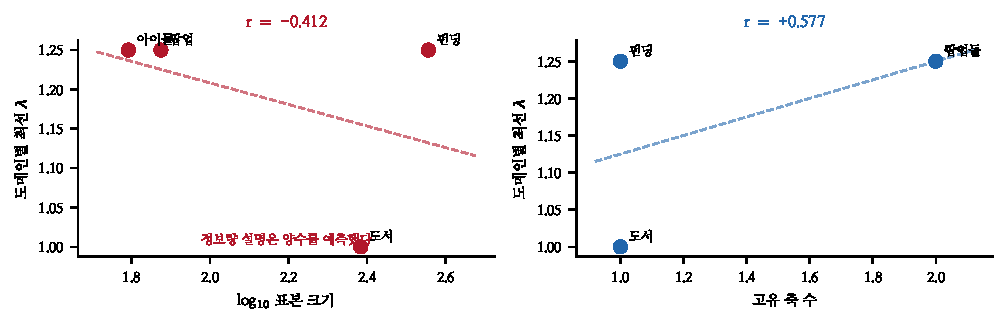
\includegraphics[width=\textwidth]{figs/lawtest.pdf}
\caption{도메인별 최선 $\lambda$와 두 설명 변수.}
\end{figure}

\begin{table}[t]
\centering\tsize
\caption{도메인별 최선 $\lambda$.}
\begin{tabular}{lrrr}
\toprule
도메인 & n & 고유 축 & 최선 $\lambda$ \\
\midrule
아이돌 & 62 & 2 & 1.25 \\
팝업 & 75 & 2 & 1.25 \\
도서 & 242 & 1 & 1.00 \\
펀딩 & 360 & 1 & 1.25 \\
\midrule
\multicolumn{2}{l}{log$_{10}$(n)과의 상관} & & \textbf{$-$0.412} \\
\multicolumn{2}{l}{고유 축 수와의 상관} & & $+$0.577 \\
\bottomrule
\end{tabular}
\end{table}

부호가 반대다. \textbf{정보량 설명은 반증됐다.} 그리고 도메인별 최선이 전부
1.0--1.25로, 노트 41이 채택한 1.5가 아니다.

\section{전이 상관이 움직이지 않는다}

왜 1.5가 19/20을 냈는지 보려고 아이돌 하나만 붙잡고 $\lambda$를 훑었다.

\begin{figure}[t]
\centering

\includegraphics[width=\textwidth]{figs/flat.pdf}
\caption{아이돌을 출처로 쓴 네 방향. 왼쪽이 순위 성능, 오른쪽이 눈금이다.}
\end{figure}

\begin{table}[t]
\centering\tsize
\caption{아이돌 출처 $\lambda$에 따른 전이 상관.}
\begin{tabular}{lrrrr}
\toprule
대상 & $\lambda{=}1.0$ & 1.25 & 1.5 & 2.0 \\
\midrule
팝업 & $+$0.458 & $+$0.458 & $+$0.457 & $+$0.458 \\
게임 & $+$0.295 & $+$0.299 & $+$0.298 & $+$0.295 \\
도서 & $+$0.269 & $+$0.269 & $+$0.269 & $+$0.269 \\
펀딩 & $+$0.225 & $+$0.226 & $+$0.227 & $+$0.228 \\
\bottomrule
\end{tabular}
\end{table}

\begin{table}[t]
\centering\tsize
\caption{같은 조건에서 예측 SD $\div$ 대상 $y$ SD.}
\begin{tabular}{lrrrr}
\toprule
대상 & $\lambda{=}1.0$ & 1.25 & 1.5 & 2.0 \\
\midrule
팝업 & 0.67 & 0.59 & 0.51 & 0.38 \\
게임 & 0.52 & 0.46 & 0.39 & 0.29 \\
도서 & 0.59 & 0.52 & 0.45 & 0.33 \\
펀딩 & 0.59 & 0.53 & 0.45 & 0.34 \\
\bottomrule
\end{tabular}
\end{table}

순위 성능은 소수점 셋째 자리에서만 흔들리고, 눈금은 절반 가까이 줄어든다.
전체 스무 셀에서 확인해도 같다 --- $\lambda$를 0.5에서 3.0까지 훑을 때 평균
전이 상관이 0.381에서 0.387 사이이고 셀별 표준편차 평균이 0.004다.

\claimx{$\lambda$는 전이의 순위 성능을 바꾸지 않는다. 바꾸는 것은 예측의 눈금이며,
$\lambda$가 커지면 인자 공간 분산이 커져 능형 계수가 작아지고 예측이 덜 퍼진다.
노트 41의 19/20은 전이가 좋아진 것이 아니라 눈금이 맞은 것이다.}{순위 성능이
$\lambda$에 반응하는 도메인 쌍이 나오면 이 진단이 좁은 것이다.}

대상 라벨은 도메인 안에서 표준화돼 SD가 1이다. 전이 상관이 $r$이면 MAE를
최소화하는 예측 스케일은 $r$ 근처다(회귀 축소). 상관이 0.27--0.46인데 예측이
0.67로 퍼져 있었으니, $\lambda$를 키워 0.38까지 줄인 것이 우연히 최적에 가까워진
것이다.

\section{축소를 명시적으로 걸어 봤다}

$\lambda$로 돌려 맞출 것이 아니라 예측을 표준화한 뒤 계수 $c$로 다시 펴면 된다.
순열 귀무분포도 같은 처리를 받게 했다.

\begin{figure}[t]
\centering
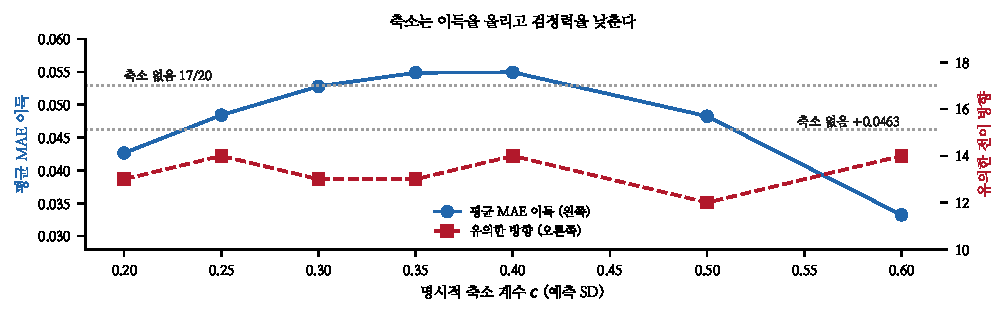
\includegraphics[width=\textwidth]{figs/metrics.pdf}
\caption{명시적 축소 계수에 따른 두 지표. 점선이 축소 없는 현행이다.}
\end{figure}

\begin{table}[t]
\centering\tsize
\caption{명시적 축소.}
\begin{tabular}{lrr}
\toprule
축소 계수 $c$ & 유의 & 평균 이득 \\
\midrule
없음(현행) & \textbf{17/20} & $+$0.0463 \\
0.30 & 13/20 & $+$0.0528 \\
0.35 & 13/20 & \textbf{$+$0.0549} \\
0.40 & 14/20 & $+$0.0549 \\
0.50 & 12/20 & $+$0.0483 \\
\midrule
출처 자기상관 & 14/20 & $+$0.0393 \\
대상 자기상관$^\dagger$ & 14/20 & \textbf{$+$0.0554} \\
\bottomrule
\end{tabular}
\end{table}

{\footnotesize $^\dagger$ 대상 라벨이 필요하므로 실전에서는 못 쓴다. 상한 참고용이다.}

\textbf{이득은 18\% 오르는데 유의는 떨어진다.} 축소가 관측 예측만이 아니라
무작위 라벨로 학습한 귀무 예측도 똑같이 개선하기 때문이다. 검정력이 오르지 않는다.

\claimx{순열 검정(MAE 기준)과 전이 상관(순위 기준)은 서로 다른 것을 잰다.
눈금만 바꾸는 조작은 앞의 것을 움직이고 뒤의 것을 움직이지 않는다. 지금까지
채택 결정을 유의 개수로 해 왔는데, 그 기준은 눈금 조작에 취약하다.}{눈금을
건드리지 않는 조작에서 두 지표가 갈리면 이 구분으로도 부족하다.}

\section{무엇을 되돌렸나}

\begin{itemize}[leftmargin=1.1em,itemsep=0.2em]
\item \textbf{철회} --- 노트 41의 ``출처 $\lambda=1.5$로 19/20''. 전이 상관이
      바뀌지 않았으므로 개선이 아니다. $\lambda$를 겹침 유도값으로 되돌렸고
      현재 상태는 17/20, 평균 이득 $+$0.0463이다.
\item \textbf{철회} --- 노트 41의 ``$\lambda$는 정보량 손잡이다''. 표본 크기와
      부호가 반대다.
\item \textbf{유지} --- 노트 41이 관찰한 사실 자체(줄이면 나빠지고 키우면
      좋아진다)는 재현된다. 해석만 틀렸다.
\item \textbf{유지} --- 노트 40의 상충 법칙. 그것은 배선에 대한 것이고 이
      노트가 다룬 것은 $\lambda$다.
\end{itemize}

\begin{quote}\fontsize{9.5}{11.5}\selectfont
노트 41은 ``법칙을 손잡이로 쓴다''로 시작해 예측이 틀린 것을 확인하고 반대
방향에서 개선을 얻었다고 썼다. 실제로는 \textbf{손잡이가 다른 기계에 붙어
있었다} --- 신호가 아니라 눈금을 돌리고 있었고, 내가 쓴 자가 눈금에 반응하는
자였다.
\end{quote}

\paragraph{축소는 언제 필요한가}
순위가 목적이면 축소는 단조 변환이라 무의미하다. 절대값이 목적일 때만 필요하고,
그 자리는 노트 26·32에서 다룬 눈금 보정이다 --- 대상 도메인 8--20건을 재서
중심과 산포를 맞추는 절차. 전이 단계에서 축소로 MAE를 낮추는 것은 그 보정을
미리 반쯤 해 두는 것에 지나지 않는다.

\section{한계}

\begin{itemize}[leftmargin=1.1em,itemsep=0.15em]
\item 도메인별 최선 $\lambda$를 네 점으로 쟀고 응답 곡선이 매우 평평하다
      (팝업은 0.367--0.369). argmax가 잡음을 고를 수 있다.
\item ``전이 상관이 $\lambda$에 무관''은 현재 다섯 도메인·현재 배선에서의
      관찰이다. 고유 축이 셋 이상인 도메인이 없다.
\item 명시적 축소를 상수와 두 규칙으로만 시험했다. 셀별로 다른 $c$를 라벨 없이
      정하는 문제는 노트 32의 미해결 문제와 같은 것이다.
\item 순열 검정을 상관 기준으로 다시 짜지 않았다. 그렇게 하면 눈금에 둔감한
      검정이 되는데 이 노트에서는 하지 않았다.
\item 노트 39의 이중 배선은 유의 개수로 채택했다. 같은 취약점이 있는지 다시
      봐야 한다.
\end{itemize}

\section{다음}

\begin{enumerate}[leftmargin=1.3em,itemsep=0.15em]
\item 순열 검정을 전이 상관 기준으로 다시 짠다 --- 눈금에 둔감한 판정.
\item 그 기준으로 노트 39의 이중 배선을 재검정한다.
\item 창작자 색인 완성 $\to$ 펀딩 매장 노출도 $\to$ 20셀 재검정.
\item 순위 성능을 실제로 올리는 조작이 무엇인지 --- 지금까지 확인된 것은
      배선(노트 34·35·37)과 도메인 추가뿐이다.
\end{enumerate}

\vspace{0.6em}
\hrule height 0.3pt
\vspace{0.5em}
{\footnotesize
\textbf{참고문헌}\\[0.3em]
Hoerl, A. E., Kennard, R. W. (1970). Ridge regression: biased estimation for
nonorthogonal problems. \emph{Technometrics}, 12(1), 55--67.\\[0.15em]
Stein, C. (1956). Inadmissibility of the usual estimator for the mean of a
multivariate normal distribution. \emph{Proc. Third Berkeley Symp.}, 1, 197--206.\\[0.15em]
Copas, J. B. (1983). Regression, prediction and shrinkage. \emph{JRSS B},
45(3), 311--354.\\[0.15em]
Good, P. (2005). \emph{Permutation, Parametric, and Bootstrap Tests of
Hypotheses}, 3rd ed. Springer.\\[0.15em]
Ben-David, S. et al. (2010). A theory of learning from different domains.
\emph{Machine Learning}, 79(1--2), 151--175.
}

\end{document}
